\newpage
\section{Iteración 6: Lectura de códigos QR}

\subsection{Introducción}

El procesamiento de imágenes es una disciplina ampliamente utilizada en la actualidad en diversas aplicaciones, que van desde la visión artificial en vehículos autónomos hasta el reconocimiento facial en dispositivos móviles. Su aplicación permite extraer información valiosa de imágenes para la toma de decisiones automatizadas.

En el contexto de esta iteración, nos enfocamos en la captura y análisis de imágenes para la detección de códigos QR. Este proceso es fundamental para la intervención en la navegación del robot, ya que le permite recibir y procesar información del entorno de manera eficiente. La integración de este sistema representa un avance significativo en la capacidad del robot para interactuar con su entorno y mejorar su movilidad.

\subsection{Requerimientos}
En esta iteración abordaremos los siguientes requerimientos funcionales:

\begin{center}
    \begin{tabular} {
        | >{\centering\arraybackslash}m{1cm}
        | >{\centering\arraybackslash}m{13cm} |}
        \hline
            ID & Descripción \\
        \hline
            RF8 & Debe poder ubicarse al robot en el plano de forma precisa \\
        \hline
            RF9 & El robot debe identificar su ambiente mediante el uso de una cámara \\ 
        \hline
    \end{tabular}
\end{center}

    Por otra parte, los requerimientos no funcionales que abordaremos son:

\begin{center}
    \begin{tabular} {
        | >{\centering\arraybackslash}m{1cm}
        | >{\centering\arraybackslash}m{13cm} |}
        \hline
            ID & Descripción \\
        \hline
            RNF1 & Debería tener tiempos de respuesta aceptables para el buen funcionamiento del sistema de control \\
        \hline
    \end{tabular}
\end{center}

\subsection{Desarrollo}

\input{iteraciones_desarrollo/iteracion_6/medición_imagenes}

\input{iteraciones_desarrollo/iteracion_6/códigos_qr}

\subsubsection{Intervención en la estimación de posición del robot}

Mencionamos anteriormente que el payload de los códigos QR contienen las coordenadas en el eje $X$e $Y$ en donde se encuentra el QR en el mapa. Al medir la distancia hacia el código lo que estamos haciendo es sumarle precisión a la determinación de la ubicación del robot. Entonces si tomamos como ejemplo ideal a una fotografía donde el código QR se encuentra perfectamente centrado, significa que el robot no presenta desplazamiento alguno el eje $X$.

\begin{figure}[H]
   \centering
   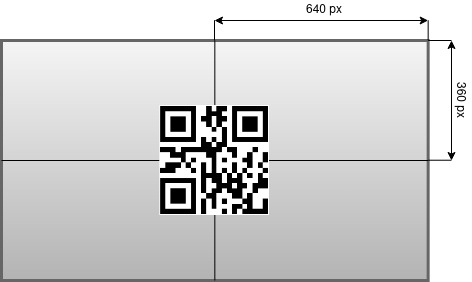
\includegraphics[width=0.7\linewidth]{images/ejemplo_foto_centro.jpg}
   \caption{Ejemplo de una fotografía con el código QR centrado}
   \label{fig:ejemplo_foto_centro}
\end{figure}

Entonces si nos basamos en la Figura \ref{fig:ejemplo_foto_centro} para determinar la posición del robot, obtenemos una posición mas precisa ya que si durante el procesamiento de la fotografía verificamos que el código QR se encuentra desplazado hacía la derecha, el robot va a estar desplazado hacía la izquierda sobre el eje $X$. Y si también el código QR detectado es de mayor dimensión en la imagen, el robot se encuentra posicionado más cerca del código QR.

Además cómo se mencionó mas arriba, el contenido del payload incluye las coordenadas en donde se encuentra el código dentro del plano. Entonces si tenemos el ejemplo donde un robot posicionado en la coordenada $(4,2)$ desea llegar a la coordenada $(4,0)$ donde se encuentra ubicado un código QR con las coordenadas descritas, nos encontramos en la situación en la que, por su posición actual, le es imposible al robot reconocer el código QR por la gran distancia que existe entre él y la cámara del robot, por lo tanto estimamos que el robot mientras realiza desplazamientos entre celda y celda siempre va a terminar posicionado al centro de ella.

\begin{figure}[H]
   \centering
   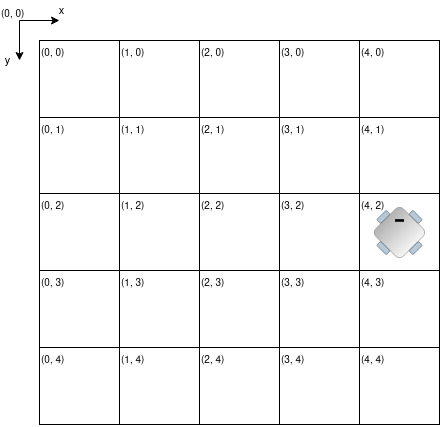
\includegraphics[width=0.5\linewidth]{images/robot_posicion_0.jpg}
   \caption{Robot posicionado en la coordenada $(4,2)$}
   \label{fig:robot_posicion_0}
\end{figure}

Ahora si el robot se encuentra llegando a su destino, la coordenada $(4,0)$ y se encuentra dentro del rango de distancia de reconocimiento de códigos QR, va a calcular la distancia tanto en el eje $Y$ como en el $X$ y sumarla al payload del código QR para después poder reportar esa coordenada. Entonces en ese momento, así como muestra la figura \ref{fig:robot_posicion_1} el robot en realidad se encuentra ubicado en la coordenada $(4.2,0.5)$ y no el centro de la celda como uno supone cuando no tiene el reporte de su ubicación en todo momento.

\begin{figure}[H]
   \centering
   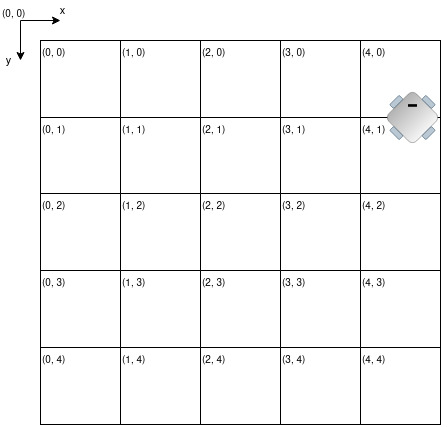
\includegraphics[width=0.5\linewidth]{images/robot_posicion_1.jpg}
   \caption{Robot posicionado en la coordenada $(4.2,0.5)$}
   \label{fig:robot_posicion_1}
\end{figure}

La siguiente imagen \ref{fig:qrcamararobot} muestra cómo es una fotografía captada en movimiento por el robot y la lectura que hace del payload, cómo se puede observar es una imagen bastante nítida y con buen enfoque lo que permite que el procesamiento de la misma se realice con mayor precisión.

\begin{figure}[H]
   \centering
   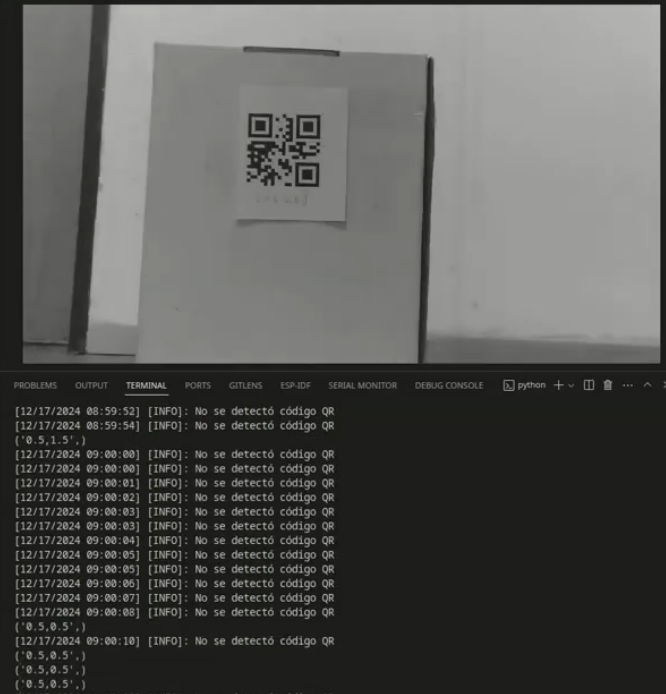
\includegraphics[width=0.7\linewidth]{images/qr.png}
   \caption{Imagen obtenida por el robot en movimiento}
   \label{fig:qrcamararobot}
\end{figure}

\subsection{Pruebas y testing}

\begin{testtableformat}
   \hline \rowcolor{test_header_color}
       Test ID             & TC\_06\_00 \\
   \hline
       Tipo de test        & Test unitario \\
   \hline
       Objeto de prueba    & Calibración de la cámara \\
   \hline
       Requerimiento       & RF4 \\
   \hline
       Nombre              & Medición de la distancia hacia un objetivo \\
   \hline
       Descripción         & Lograr capturar la fotografía de un objetivo en un ambiente controlado para tomar obtener los parámetros de calibración de la cámara.\\
   \hline
       Precondición        & PRECOND\_H\\
   \hline
       Pasos del test      & \begin{enumerate}
                             \item Capturar una fotografía con la ESP32-CAM.
                             \item Envíar la imagen por comunicación inalámbrica hacia el servidor que aloja la imagen.
                             \item Verificar que la imagen llegó completa.
                             \item Procesar la imagen para obtener los parámetros de la imagen.
                             \end{enumerate} \\
   \hline
       Resultado esperado  & La imagen debe llegar de forma completa y en el procesamiento se debe detectar el código QR. \\
   \hline
       Resultado obtenido  & Tanto la imagen como el procesamiento fueron obtenidas de forma correcta. \\
   \hline
       Observaciones       & - \\
   \hline
\end{testtableformat}

\begin{testtableformat}
   \hline \rowcolor{test_header_color}
       Test ID             & TC\_06\_01 \\
   \hline
       Tipo de test        & Test unitario \\
   \hline
       Objeto de prueba    & Envío del contenido del payload \\
   \hline
       Requerimiento       & RF4 \\
   \hline
       Nombre              & Coordenadas del payload \\
   \hline
       Descripción         & Capturar una fotografía, detectar si existe un código QR en la imagen y enviar el contenido del payload.\\
   \hline
       Precondición        & PRECOND\_H\\
   \hline
       Pasos del test      & \begin{enumerate}
                             \item Capturar una fotografía con la ESP32-CAM.
                             \item Enviar la imagen por comunicación inalámbrica hacia el servidor que aloja la imagen.
                             \item Verificar que la imagen llegó completa.
                             \item Procesar la imagen para obtener los parámetros de la imagen.
                             \end{enumerate} \\
   \hline
       Resultado esperado  & Se debe poder llegar a leer el payload de forma completa. \\
   \hline
       Resultado obtenido  & El contenido del payload se lee correctamente. \\
   \hline
       Observaciones       & - \\
   \hline
\end{testtableformat}

\begin{testtableformat}
    \hline \rowcolor{test_header_color}
        Test ID             & TC\_06\_02 \\
    \hline
        Tipo de test        & Test unitario \\
    \hline
        Objeto de prueba    & Determinar la distancia máxima de reconocimiento del código QR \\
    \hline
        Requerimiento       & RF4 \\
    \hline
        Nombre              & Máxima distancia \\
    \hline
        Descripción         & Capturar fotografías a diferentes distancias, detectar si existe un código QR en la imagen y enviar el contenido del payload\\
    \hline
        Precondición        & PRECOND\_H\\
    \hline
        Pasos del test      & \begin{enumerate}
                              \item Colocar el robot con la cámara a una distancia conocida del código QR
                              \item Capturar una fotografía con la ESP32-CAM
                              \item Enviar la imagen por comunicación inalámbrica hacia el servidor que aloja la imagen
                              \item Verificar que la imagen llegó completa
                              \item Procesar la imagen para obtener los parámetros de la imagen
                              \item Repetir los pasos desde el 1) hasta encontrar la distancia máxima de reconocimiento
                              \end{enumerate} \\
    \hline
        Resultado esperado  & Se debe poder llegar a leer el payload de forma completa, si es que no se lee el contenido del payload encontrar la distancia máxima de reconocimiento \\
    \hline
        Resultado obtenido  & El contenido del payload se lee correctamente a una distancia máxima de 600 milímetros\\
    \hline
        Observaciones       & - \\
    \hline
 \end{testtableformat}

\begin{testtableformat}
   \hline \rowcolor{test_header_color}
       Test ID             & TC\_06\_03 \\
   \hline
       Tipo de test        & Test integración \\
   \hline
       Objeto de prueba    & Realizar procesamiento de los códigos QR mientras el robot se encuentra en movimiento\\
   \hline
       Nombre              & Captura de fotografías con el robot en movimiento\\
   \hline
       Descripción         & La idea es capturar y enviar las fotografías de los códigos QR que se encuentran dispersos a lo largo del mapa mientras el robot realiza un desplazamiento\\
   \hline
       Precondición        & PRECOND\_H \\
   \hline
       Pasos del test      & \begin{enumerate}
                             \item Validar que se reciben las fotografías
                             \item Inicializar el proceso de desplazamiento del robot
                             \item Capturar y envíar las fotografías tomadas
                             \item Validar que el procesamiento de las fotos es correcto y el payload es legible
                             \end{enumerate} \\
   \hline
       Resultado esperado  & Recibir las fotografías de forma correcta y realizar la lectura y procesamiento del payload\\
   \hline
       Resultado obtenido  & Todas las fotos se reciben de forma completa, es decir, no contienen errores y por lo tanto el procesamiento de los códigos QR es efectiva y la información contenida en su payload es procesable\\
   \hline
       Observaciones       & - \\
   \hline
\end{testtableformat}

\begin{testtableformat}
    \hline \rowcolor{test_header_color}
        Test ID             & TC\_06\_04 \\
    \hline
        Tipo de test        & Test de sistema \\
    \hline
        Objeto de prueba    & Comunicación inalámbrica - PID - Modelo cinemático compensado - Odometría - Seguidor de línea magnética - Modelo del Mapa - Calculador de trayectorias - Interfaz de usuario - Red de Petri - Monitor - Filtro de Kalman - Lectura de códigos QR\\
    \hline
        Nombre              & Prueba de sistema integrado\\
    \hline
        Descripción         & Verificar que la interfaz, el robot y todos los componentes involucrados funcionan de manera adecuada\\
    \hline
        Precondición        & PRECOND\_I \\
    \hline
        Pasos del test      & \begin{enumerate}
                              \item En la interfaz determinar la coordenada origen y destino
                              \item Calcular la trayectorias
                              \item Enviar los setpoints
                              \item Comprobar que el robot se mueve a lo largo de la trayectoria definida, al desviarse se corrige su posición y reporta la lectura de los códigos QR
                              \item Repetir la prueba desde el paso 1 con distintos valores
                              \end{enumerate} \\
    \hline
        Resultado esperado  & El robot pueda completar el desplazamiento definido por el usuario usando la interfaz como medio de control y el robot pueda reportar la lectura de los códigos QR de manera efectiva\\
    \hline
        Resultado obtenido  & El robot y la interfaz se comportan de manera esperada. El robot realiza las trayectorias dentro de los límites observados en las pruebas unitarias y de integración hechas anteriormente\\
    \hline
        Observaciones       & - \\
    \hline
\end{testtableformat}

\subsection{Resultados}
Los resultados son satisfactorios ya que se pudo cumplir con creces el objetivo de poder enviar y realizar el procesamiento de las imágenes tomadas por la cámara del microcontrolador ESP-32. Como este microcontrolador sólo se encarga de tomar fotos, pudimos generar imágenes de gran calidad llegando a una resolución HD y a una frecuencia de envío de 2 FPS (Frame per second), es decir, 2 imágenes por segundos. Por supuesto esto no llega a ser un procesamiento de video ya que no se arma un objeto con esas imágenes, solamente se realiza el procesamiento de las mismas de forma particular.
Además no implicó realizar cambios grandes en el sistema principal de movilización del robot, esto porque al estar todo conectado vía las comunicaciones inalámbricas, el sistema explicado puede considerarse como un módulo externo, que, por supuesto ayuda al robot a tomar conocimiento de su entorno.

\subsection{Riesgos superados}

En esta iteración se demostró que los nuevos componentes integrados al sistema, como ser el microcontrolador ESP32-CAM, el procesamiento de imágenes y la medición de distancia hacia códigos QR, interactúan de forma correcta con los componentes ya desarrollados en las iteraciones anteriores, y por lo tanto se supera efectivamente el riesgo representado por RI-02.

\begin{center}
    \begin{tabular} {
        | c| c |}
        \hline \rowcolor{test_header_color}
            ID & Riesgo \\
        \hline
            RI-02 & Intercomunicación de componentes ineficiente o ineficaz \\
        \hline
    \end{tabular}
\end{center}

\subsection{Conclusiones}
En este capítulo se explicaron los motivos que nos llevaron a implementar este tipo de procesamiento y porque consideramos que el conocimiento del entorno y sus parámetros son importantes para mejorar la movilización del robot en un entorno real. Lamentablemente, los tiempos del proyecto no fueron suficientes para realizar todas las pruebas necesarias y verificar fehacientemente que el comportamiento del robot cambian para mejor con la ayuda de las mediciones tomadas de las imágenes, esto teniendo en cuenta que no se añaden de forma directa ni se suman como entrada al filtro de Kalman.
Esperamos que una próxima iteración de la serie Hermes esto se pueda continuar, y plasmar en el mundo real lo que planteamos en la teoría de la implementación.